\documentclass{article}

% Informations

% Modules 
\usepackage[greek,english,french]{babel}
\usepackage{graphicx}						% Gestion des images
\usepackage{caption}                        % Gestion des titres
\usepackage{appendix}                       % Gestion de l'annexe
\usepackage[utf8]{inputenc}                 % Encodage du texte
\usepackage{multicol}                       % Gestion des multi-colonnes des tableaux
\usepackage{booktabs}                       % Importation des traits horizontaux des tableaux
\usepackage{siunitx}                        % Gestion des unités
\usepackage{mwe,lipsum}                     % Modules de Minimal Working Examples
\usepackage{amsmath,amssymb,amsbsy}         % Ajout d'options dans le mode 'math'
\usepackage{todonotes}                      % Ajout des notes en marge
\usepackage{mathtools}                      % Autres outils pour le mode 'math'
\usepackage[a4paper]{geometry}                       % Options de mise en page
\usepackage{listings}
\usepackage{color,xcolor}
\usepackage{csquotes}
\usepackage{textcomp}
\usepackage{fancyhdr}
\usepackage{lmodern}
\usepackage[T1]{fontenc}
\usepackage{lato}
\usepackage{titling}
\usepackage{datetime}
\usepackage[version=4]{mhchem}
\usepackage{pdfpages}

% Police d'écriture
\renewcommand\familydefault{\sfdefault}

% Définition de couleurs
\definecolor{Bleu_ENSPS}{RGB}{0,119,139}
\usepackage[colorlinks=true,allcolors=Bleu_ENSPS]{hyperref} 

% Options de format pour les unités (SIUnitX package)
\sisetup{
    detect-all,
    locale                  = FR,
    sticky-per,
    inter-unit-product      = {.},
    per-mode                = reciprocal-positive-first,
}

\DeclareSIUnit\octet{o}
\DeclareSIUnit\euro{€}

%Options de largeur de marges, verticales et horizontales
\geometry{hmargin=3cm,vmargin=2cm}
\setlength{\parindent}{7mm}

% Mise en page
\pagestyle{fancy}
\setlength{\headheight}{14pt}
\renewcommand\headrulewidth{0.5pt}
\renewcommand\footrulewidth{0.5pt}
\fancyhead[C]{\thedate}
\fancyhead[R]{}%\rightmark
\fancyhead[L]{}

% Bibliographie
\usepackage[style=authoryear,giveninits=true,sorting=nty]{biblatex}
\DefineBibliographyExtras{french}{\restorecommand\mkbibnamefamily}

\AtEveryBibitem{%
  \clearlist{language}%
  \clearlist{urldate}
  \clearlist{url}
  \clearfield{month}
  \clearfield{day}
}
\DeclareFieldFormat{url}{}
\DeclareFieldFormat{urldate}{}

\DeclareFieldFormat{journaltitle}{\textit{#1}}
\DeclareFieldFormat{title}{#1}

\setlength\bibitemsep{\itemsep}
\AtEveryCite{\color{Bleu_ENSPS}}

\addbibresource{/home/amounier/Documents/Bibliographie/bibliographie_bib.bib}
\bibliography{biblatex-examples.bib}

% All name in hyperlink (cite biblatex)
\makeatletter
\let\abx@macro@citeOrig\abx@macro@cite
\renewbibmacro{cite}{%
   \bibhyperref{%
   \let\bibhyperref\relax\relax%
   \abx@macro@citeOrig%
   }%
}
\let\abx@macro@textciteOrig\abx@macro@textcite
\renewbibmacro{textcite}{%
   \bibhyperref{%
   \let\bibhyperref\relax\relax%
   \abx@macro@textciteOrig%
   }%
}%
\makeatother

% Passage des mots table et figure dans les lien hypertextes
\makeatletter
\renewcommand\p@table{Table~\@ }
\renewcommand\p@figure{Figure~\@ }
\makeatother

\newcounter{includepdfpage}

% Styles équations
%\numberwithin{equation}{section}

%Autres commandes
% \newcommand{\CO}{\ce{CO_2}}

% Titre ---------------------------------------
\date{\today}
\title{Dossier de demande de remboursement}
\author{\href{mailto:prenom.nom@mail.fr}{Prénom Nom}}

% Informations --------------------------------
\newcommand\remboursementMotif{Motif de remboursement}
\newdate{remboursementDate}{28}{01}{2026}

\begin{document}

\centerline{\huge \noindent \thetitle}

\vspace{3mm}
{\Large \noindent \theauthor}

\vspace{8mm}

\noindent
{\remboursementMotif, le \displaydate{remboursementDate}.}\\

\noindent
Demande de remboursement :
\begin{table}[ht]
   \centering
   \begin{tabular}{cllr}
      & Hôtel & (page \ref{hotel}) & \SI{120}{\euro} \\
      + & Train & (page \ref{train}) & \SI{288}{\euro} \\
      + & Repas & (page \ref{repas}) & \SI{16.8}{\euro} \\
      \midrule
      Total & & & \SI{424.8}{\euro} \\
   \end{tabular}
\end{table}

\noindent
Relevé d'identité bancaire inclus au dossier, page \ref{rib}.

\phantom{\addtocounter{includepdfpage}{1}\theincludepdfpage}

\newpage
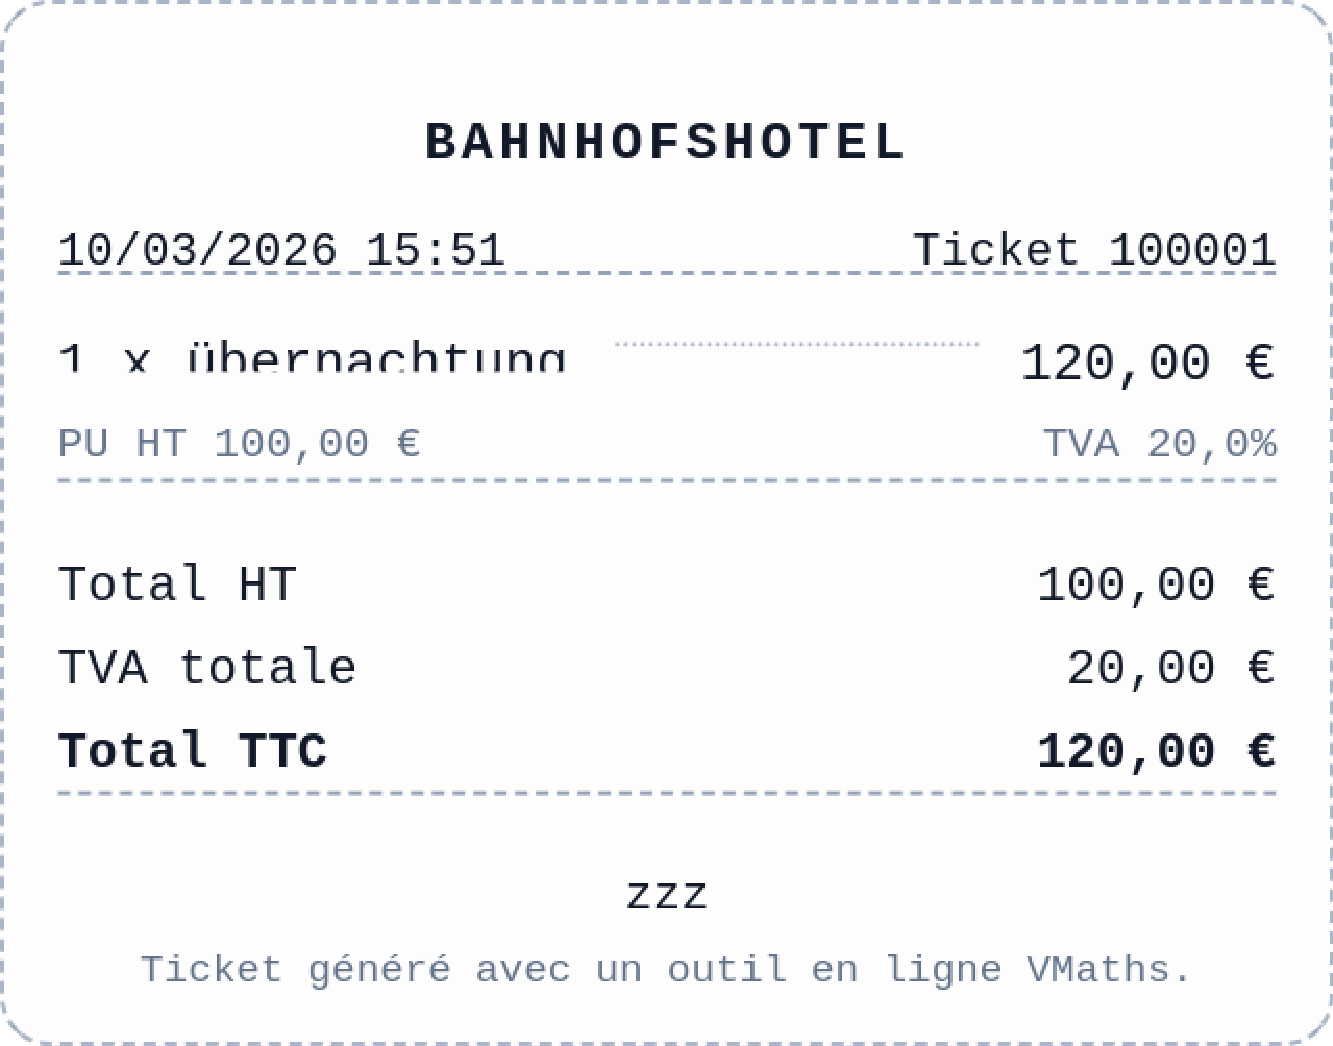
\includepdf[pages={1},link,linkname=hotel,pagecommand={\refstepcounter{includepdfpage}\label{hotel}}]{documents/ticket_caisse_hotel.pdf}

\newpage
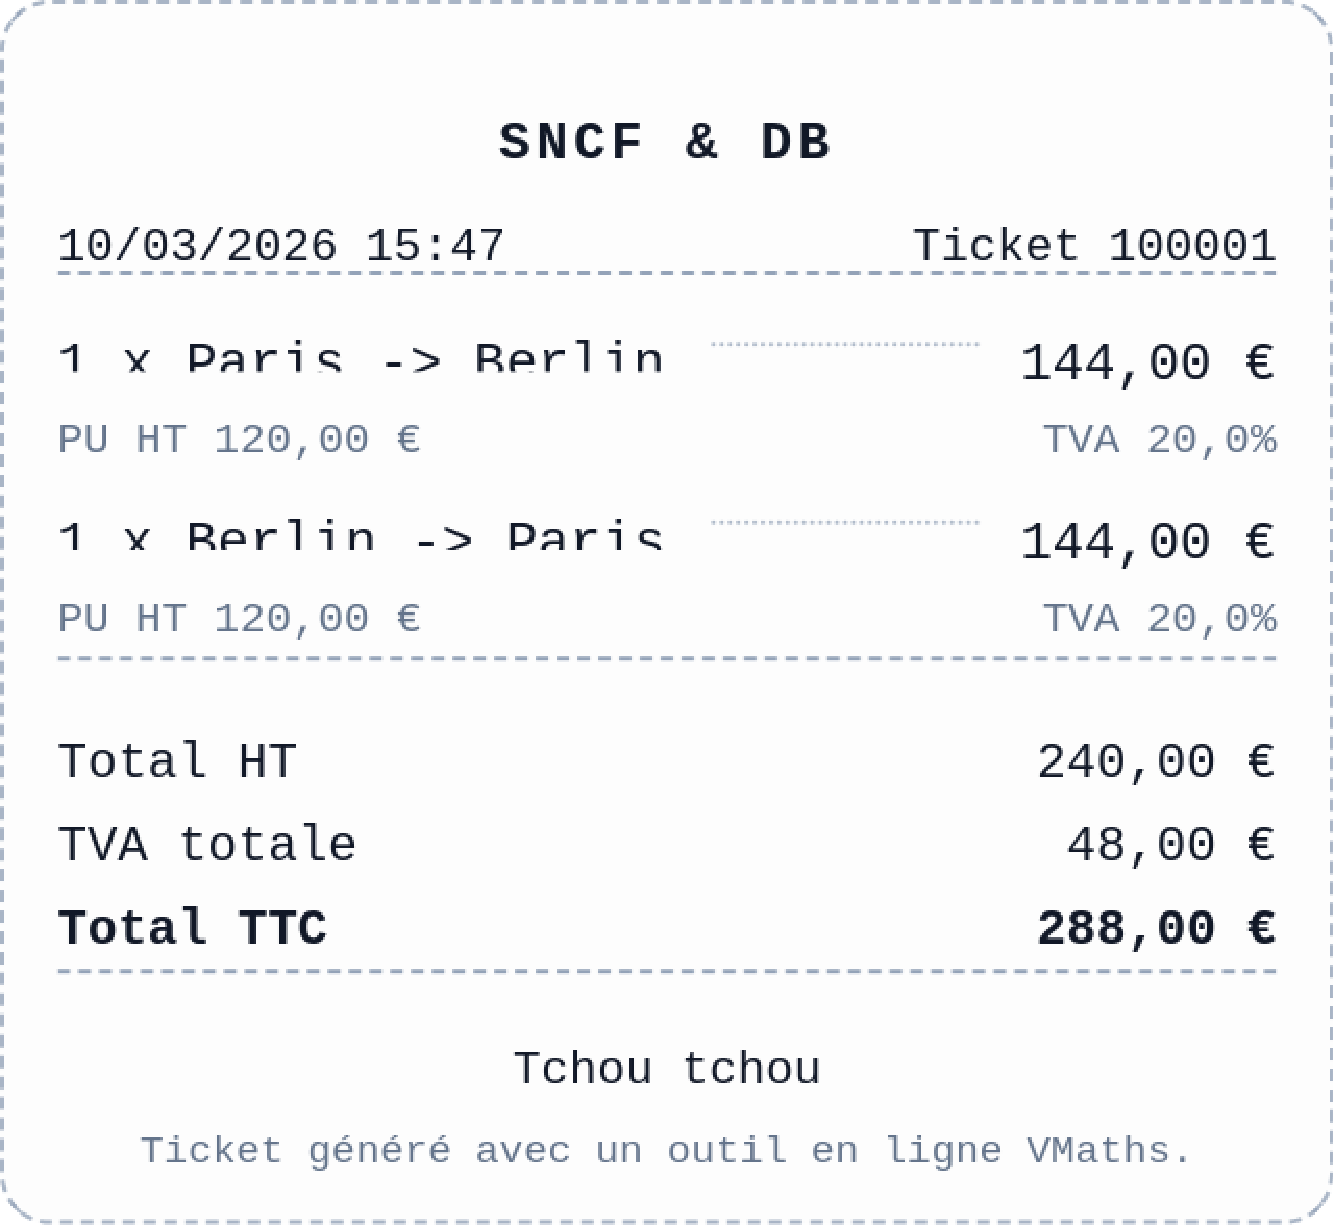
\includepdf[pages={1},link,linkname=train,pagecommand={\refstepcounter{includepdfpage}\label{train}}]{documents/ticket_caisse_train.pdf}

\newpage
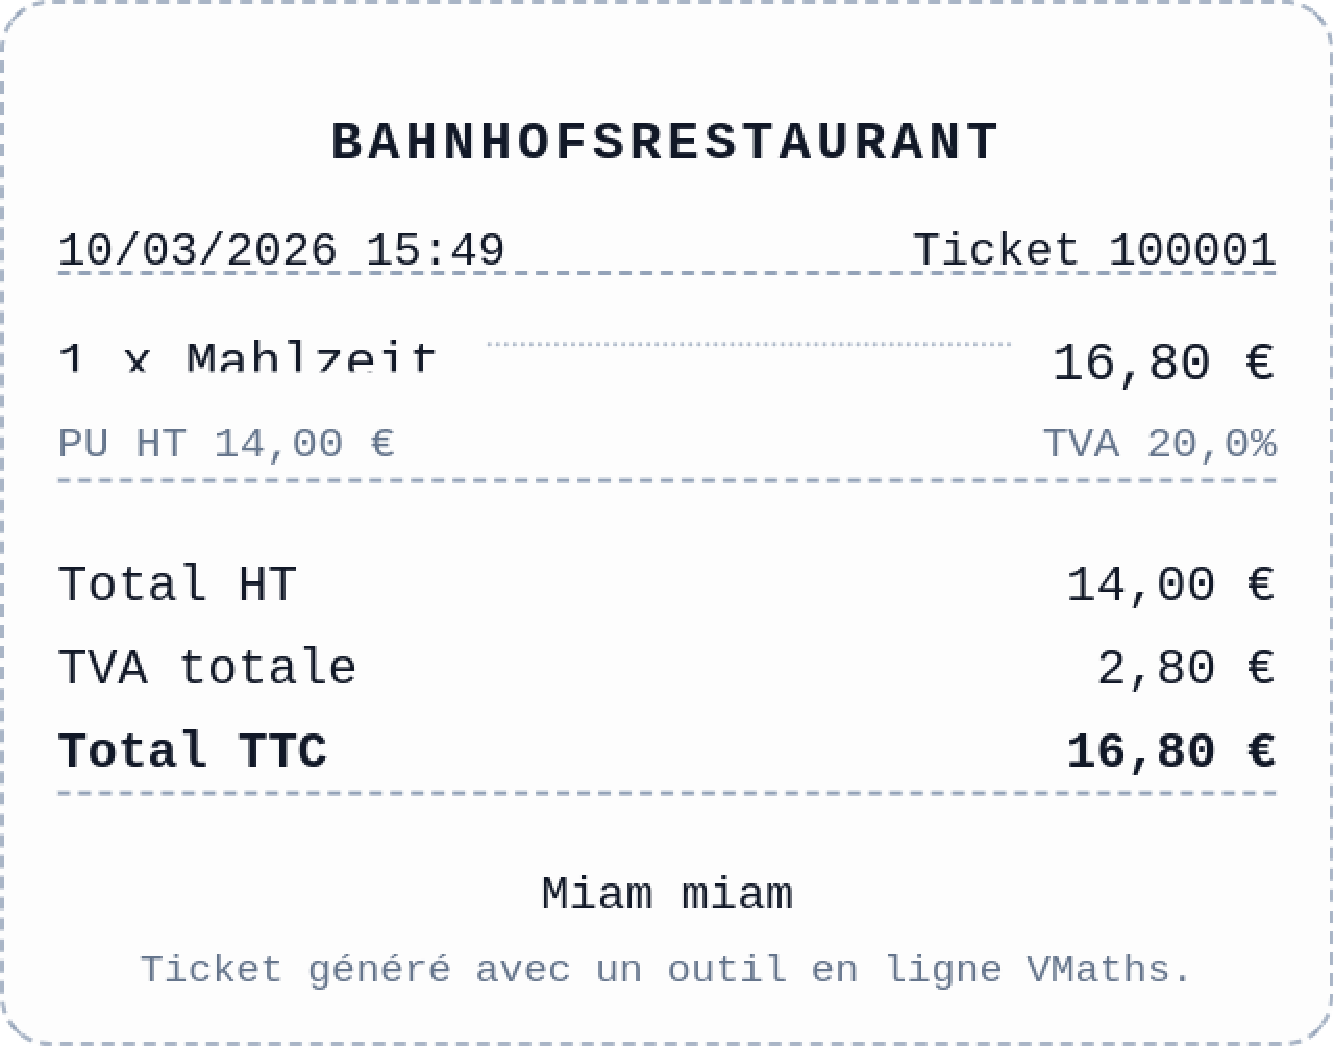
\includepdf[pages={1},link,linkname=repas,pagecommand={\refstepcounter{includepdfpage}\label{repas}}]{documents/ticket_caisse_repas.pdf}

\newpage
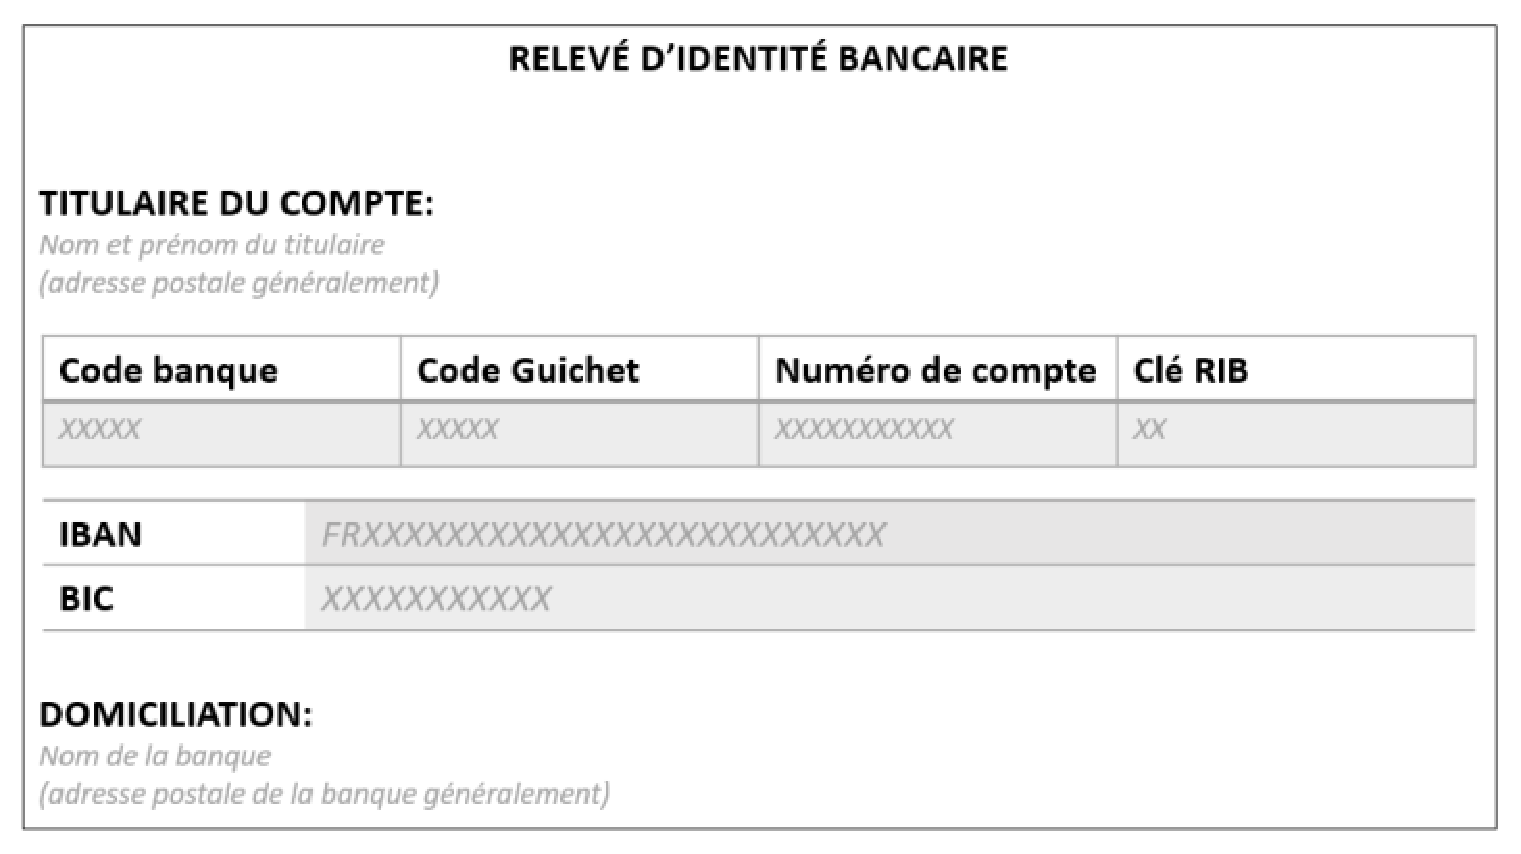
\includepdf[pages={1}, link,linkname=rib,pagecommand={\refstepcounter{includepdfpage}\label{rib}}]{documents/rib.pdf}
\end{document}
